\section{Preparação dos modelos}
\label{sec:metodologia-preparacao-modelos}

% Uma vez que temos um \textit{dataset} com atributos fonológicos processados, agora podemos prosseguir com a preparação das features e dos modelos para reconhecimentos dos sinais utilizando a abordagem proposta.


% Experimento
%   Preparação das features (asl-phono -> palavras)
%       Transformação das sequências no dataset: frames -> palavras
%       Justificativa??
%   Preparação dos modelos (Transformer, LSTM, GRU, etc) -- por modelo
%       Arquitetura + Parâmetros
%       lr scheduler, optimizer, loss function
%       Busca de parâmetros (dimensionar os modelos/parâmetros)



% SELEÇÃO DOS MODELOS -------------------------------------------

Tomando como referência a discussão introduzida na \autoref{sec:modelos-sequenciais}, adotaremos nos experimentos deste trabalho três das principais arquiteturas utilizadas em tarefas de \acrfull{nlp}: o \textit{Encoder-Decoder} em uma versão com \acrfull{lstm} e em outra com \acrfull{gru}, e também o \textit{Transformer}.

% Os parâmetros para treinamento dos modelos foram selecionados com base na discussão apresentada por \citeonline{goodfellow-2016-deep-learning}, a qual aborda de forma prática temas como definição de métricas, modelos de base, otimização de parâmetros, entre outros para tal finalidade.

Para estabelecer os parâmetros dessas arquiteturas, as estratégias de otimização e treinamento, bem como as métricas a serem utilizadas nos experimentos, nos fundamentamos pela discussão apresentada por \citeonline{goodfellow-2016-deep-learning}.
Dessa forma, o algoritmo de otimização será definido como o \acrfull{sgd} com \textit{momentum} de 0,9. Ele será combinado a uma estratégia de redução da taxa de aprendizagem por um fator de 0,2 sempre que o valor da perda calculada sobre os dados de validação atingir um platô por 5 épocas seguidas. A função de perda, por sua vez, será a \textit{Cross-Entropy Loss} (ou Perda de Entropia Cruzada) e os \textit{batches} de dados possuirão tamanho de 50 amostras. Por fim, os dados serão particionados numa proporção de 15\% para validação, 15\% para testes e o restante para treinamento dos modelos.

% Dessa forma, utilizamos como algoritmo de otimização o \acrfull{sgd} com \textit{momentum} de 0,9. Ele foi combinado com uma estratégia de redução da taxa de aprendizagem por um fator de 0,2 sempre que o valor da perda calculada sobre os dados de validação atinge um platô por 5 épocas seguidas. A função de perda utilizada, por sua vez, foi a \textit{Cross-Entropy Loss} (ou Perda de Entropia Cruzada). Além disso, adotamos \textit{batches} com tamanho de 50 amostras e particionamos o \textit{dataset} numa proporção de 15\% para validação, 15\% para testes e o restante para treinamento dos modelos.


Realizamos uma otimização de parâmetros do tipo \textit{Grid Search} para identificar a melhor configuração para cada um dos modelos em nosso contexto. 

% TODO: detalhar arquitetura do seq2seq + lstm:
Para o modelo \textit{Encoder-Decoder} com \acrshort{lstm} utilizamos ...


% \figura[]
%     {fig:otim_lr_encdec_lstm}
%     {capitulos/metodologia/imagens/otim_encdec_lstm_lr}
%     {height=4.0cm}
%     {Otimização da taxa de aprendizagem com relação à perda calculada para o \textit{Encoder-Decoder (LSTM)}. LR refere-se à taxa de aprendizagem (ou \textit{learning rate}).}
%     {}


\begin{figure}[ht!]
    \centering
    \caption{\textmd{???.}}
    \subcaptionbox{\label{subfig:otim-encdec-lstm-lr}}{
        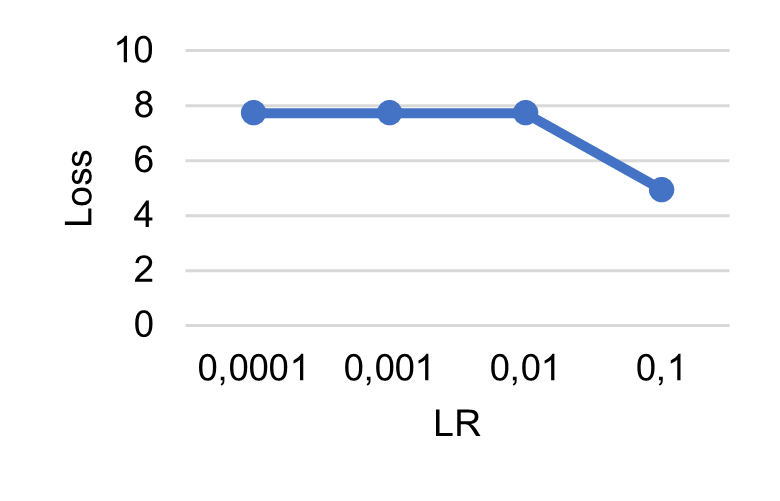
\includegraphics[width=5.0cm]{capitulos/metodologia/imagens/otim_encdec_lstm_lr}
    }%
    \hfill
    \subcaptionbox{\label{subfig:otim-encdec-lstm-dropout}}{
        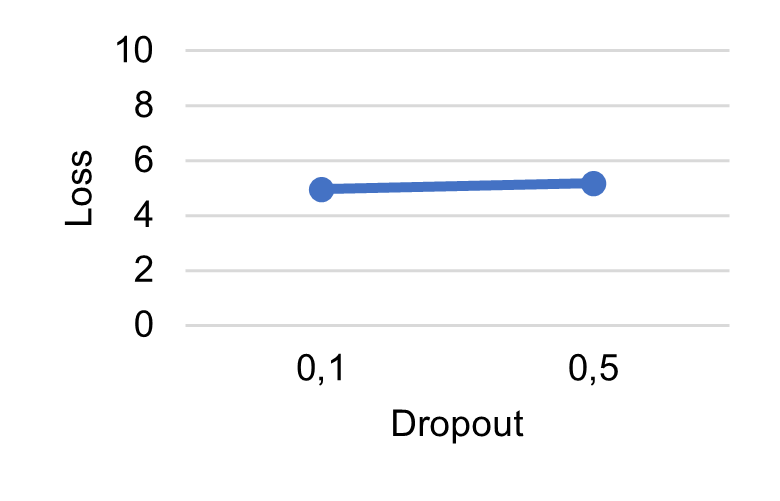
\includegraphics[width=5.0cm]{capitulos/metodologia/imagens/otim_encdec_lstm_dropout}
    }%
    \hfill
    \subcaptionbox{\label{subfig:otim-encdec-lstm-layers}}{
        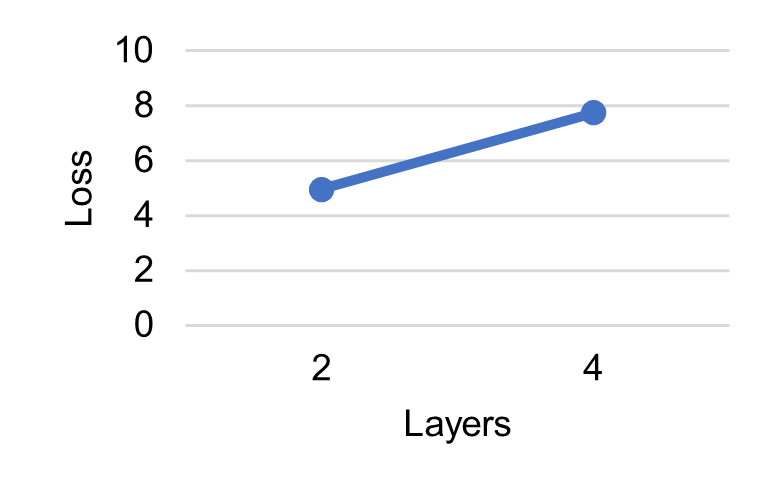
\includegraphics[width=5.0cm]{capitulos/metodologia/imagens/otim_encdec_lstm_layers}
    }%
    \hfill
    \subcaptionbox{\label{subfig:otim-encdec-lstm-hidden}}{
        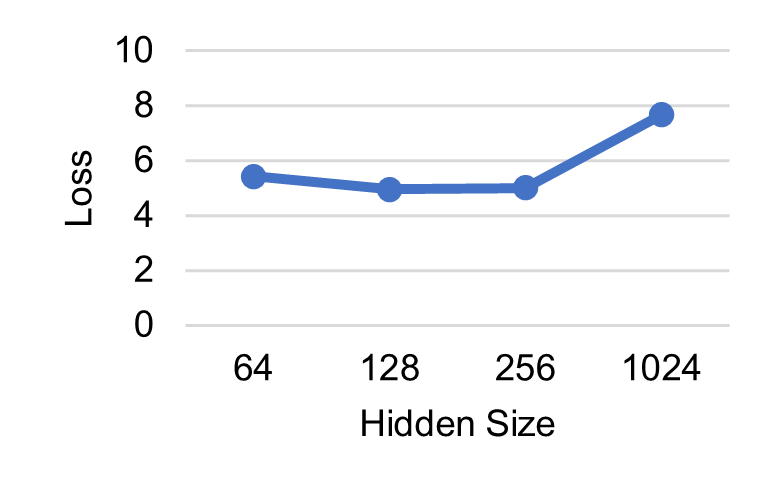
\includegraphics[width=5.0cm]{capitulos/metodologia/imagens/otim_encdec_lstm_hidden_size}
    }%
    % \hfill
    \subcaptionbox{\label{subfig:otim-encdec-lstm-emb}}{
        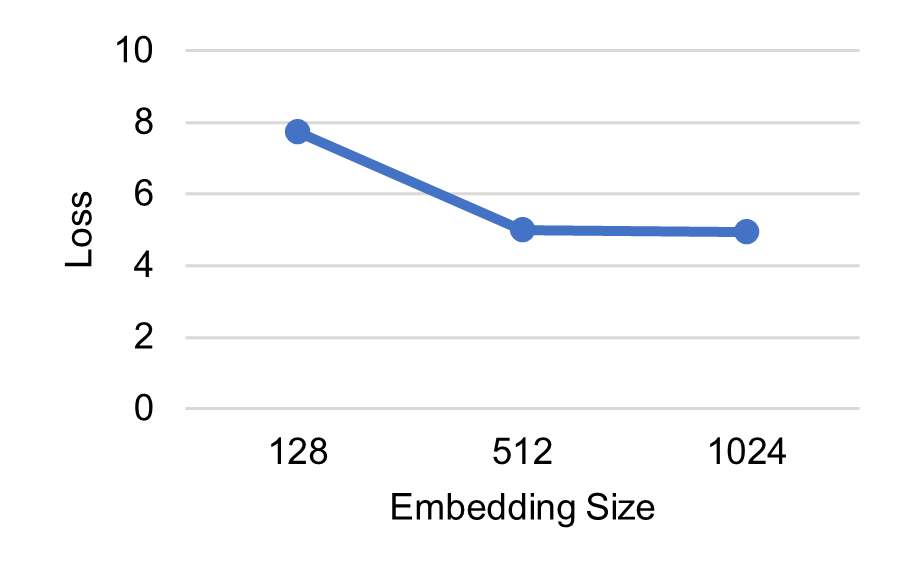
\includegraphics[width=5.0cm]{capitulos/metodologia/imagens/otim_encdec_lstm_emb_size}
    }%
    \nomefonte{}
    \label{fig:otim-encdec-lstm}
\end{figure}
    


% TODO: detalhar arquitetura do seq2seq + gru:
Para o \textit{Encoder-Decoder} com \acrshort{gru}, por sua vez, utilizamos ...


\figura[]
    {fig:otim_lr_transformer}
    {capitulos/metodologia/imagens/otim_transformer_lr}
    {height=4.0cm}
    {Otimização da taxa de aprendizagem com relação à perda calculada para o \textit{Transformer}. LR refere-se à taxa de aprendizagem (ou \textit{learning rate}).}
    {}


No caso do \textit{Transformer}, não aplicamos nenhuma customização e adotamos a arquitetura original introduzida por \citeonline{vaswani-2017-transformer} -- que consiste de \textit{embeddings} com dimensões de 512, camadas ocultas com dimensões de 2048, 6 camadas, 8 cabeças e \textit{dropout} de 0,1.
Realizamos uma otimização da taxa de aprendizagem para esse modelo utilizando a estratégia de \textit{grid search} com validação cruzada de 5 \textit{folds} por 50 épocas. O resultado, ilustrado na \autoref{fig:otim_lr_transformer}, nos mostra que o valor que melhor minimiza a perda é 0,1.

\figura[]
    {fig:otim_lr_encdec_gru}
    {capitulos/metodologia/imagens/otim_encdec_gru_lr}
    {height=4.0cm}
    {Otimização da taxa de aprendizagem com relação à perda calculada para o \textit{Encoder-Decoder (GRU)}. LR refere-se à taxa de aprendizagem (ou \textit{learning rate}).}
    {}

O código-fonte utilizado nos experimentos deste trabalho está disponível no endereço indicado abaixo\footnote{
    Disponível em \url{https://www.cin.ufpe.br/~cca5/sl-nlp}.
}.



% \cite{goodfellow-2016-deep-learning}

% --------
% A reasonable choice of optimization algorithm is SGD with momentum with a decaying learning rate (popular decay schemes that perform better or worse on different problems include decaying linearly until reaching a fixed minimum learning rate, decaying exponentially, or decreasing the learning rate by a factor of 2–10 each time validation error plateaus).

% - optimizer: SGD
%     nesterov: False
%     momentum: 0.9
% --------
% Loss function

% - criterion: CrossEntropyLoss

% --------
% Early stopping should be used almost universally.

% - training_args:
%     max_epochs: 50
%     batch_size: 50
%     lr: 0.01
%     test_size: 0.15
%     valid_size: 0.15
%     early_stopping:
%         patience: 10
%         threshold: 10e-4
%         threshold_mode: rel
%     gradient_clipping:
%         gradient_clip_value: 0.5
%     lr_scheduler: 
%         policy: ReduceLROnPlateau
%         factor: 0.2
%         patience: 5

% --------
% Learning rate - apresentar graficos?
% - learning rate (grid search)


% --------
% - dimensões dos modelos

%     Transformer (selecionamos as dimensões do modelo clássico \cite{vaswani-2017-transformer})
%         embedding_size: 512
%         hidden_size: 2048
%         num_layers: 6
%         dropout: 0.1
%         num_heads: 8

    